\documentclass[letterpaper,addpoints, 11pt]{exam}

\usepackage{graphicx}  
\usepackage{amsmath, latexsym, color, graphicx, amssymb, bm, here, enumerate}
\usepackage{epsf, epsfig, pifont,tikz,subfigure}
\usepackage{graphics, calrsfs}
\usepackage{times}
\usepackage{fancybox,calc}
\usepackage{palatino,mathpazo}
\usepackage{amsfonts}
\usepackage{wrapfig}
\usepackage{multicol}
\usepackage{sidecap}
\usepackage[colorlinks=true, urlcolor=cyan, linkcolor=cyan]{hyperref}
\usepackage{media9}
\usepackage{mathtools}
\usepackage{soul}
\usepackage{enumitem}
\usepackage[margin=0.5in, footskip=0.25in]{geometry}
\usepackage{sectsty}
\sectionfont{\centering}
\renewcommand\thesection{\Roman{section}.}
\renewcommand\thesubsection{\Alph{subsection}.}
\renewcommand\thesubsubsection{\thesubsection \arabic{subsubsection}.}
\usepackage{listings}
\usepackage{caption}
\DeclareCaptionFont{white}{\color{white}}
\DeclareCaptionFormat{listing}{%
	\parbox{\textwidth}{\colorbox{gray}{\parbox{\textwidth}{#1#2#3}}\vskip-4pt}}
\captionsetup[lstlisting]{format=listing,labelfont=white,textfont=white}
\lstset{frame=lrb,xleftmargin=\fboxsep,xrightmargin=-\fboxsep}
\usepackage{url}
\urlstyle{same}
\usepackage{wasysym}
\usepackage[export]{adjustbox}
%_______________________________________________



\begin{document}

\begin{center}
	\Large \textbf{ISA 401/501 - Business Intelligence \& Data Viz} \\
	\Large \textbf{16: An Overview of Data Viz Software (Tableau, R \& Python)} \\
\end{center}

%\vspace{5mm}
%
%\makebox[\textwidth]{Name and ID:\enspace\hrulefill}
%
%\vspace{5mm}
%
%\makebox[\textwidth]{Section:\enspace\hrulefill}

\begin{center}
	\fbox{\fbox{\parbox{\textwidth}{\centering
				\textbf{\large Learning Objectives for Today's Lab:}
				\vspace{-2mm}
				\begin{enumerate}[label=(\Alph*)]
					\item Create your first visualizations, dashboard and story map in \textbf{Tableau}.
					\item Create a virtual environment, install libraries and capitalize on the pandas-profiling and pycaret \textbf{Python} libraries for visualizing machine learning problems (exploration and post model diagnostics). 
					\item Create exploratory plots for machine learning problems in \textbf{R}.
					\item If time allows, discuss the grammar of graphics and its implementation in R and Python via the ggplot2 and plotnine libraries, respectively.
				\end{enumerate}
			}}}
		\end{center}	
%		\begin{center}
%			\addpoints
%			\combinedgradetable[h][questions]
%		\end{center}
%		
%		\newpage

\begin{questions}

\question[0] We will begin today's class with a quick discussion of \href{https://miamioh.instructure.com/courses/179812/quizzes/506303}{Assignment 11} and then, compete in a \textbf{Kahoot Competition on the Fundamentals of Data Visualization} for a \$15 Starbucks gift card. 

\vspace{0.5in}

\question[0] Let us use \textbf{Tableau} to examine Ohio's Summary Data for COVID-19 deaths (see \url{https://coronavirus.ohio.gov/static/dashboards/COVIDDeathData_CountyOfDeath.csv}). In Tableau, let us:
\begin{enumerate}[label=(\Alph*)]
	\item Create a map of the sum of measure counts by county, with a filter of different measures.
	\item Create a line-chart (as well as a time-based bar chart) for the sum of case counts for the entire state.
	\item We will then combine these two charts in a dashboard.
	\item We will also use the storyboard feature to highlight interesting aspects of the data.
\end{enumerate}

\begin{center}
	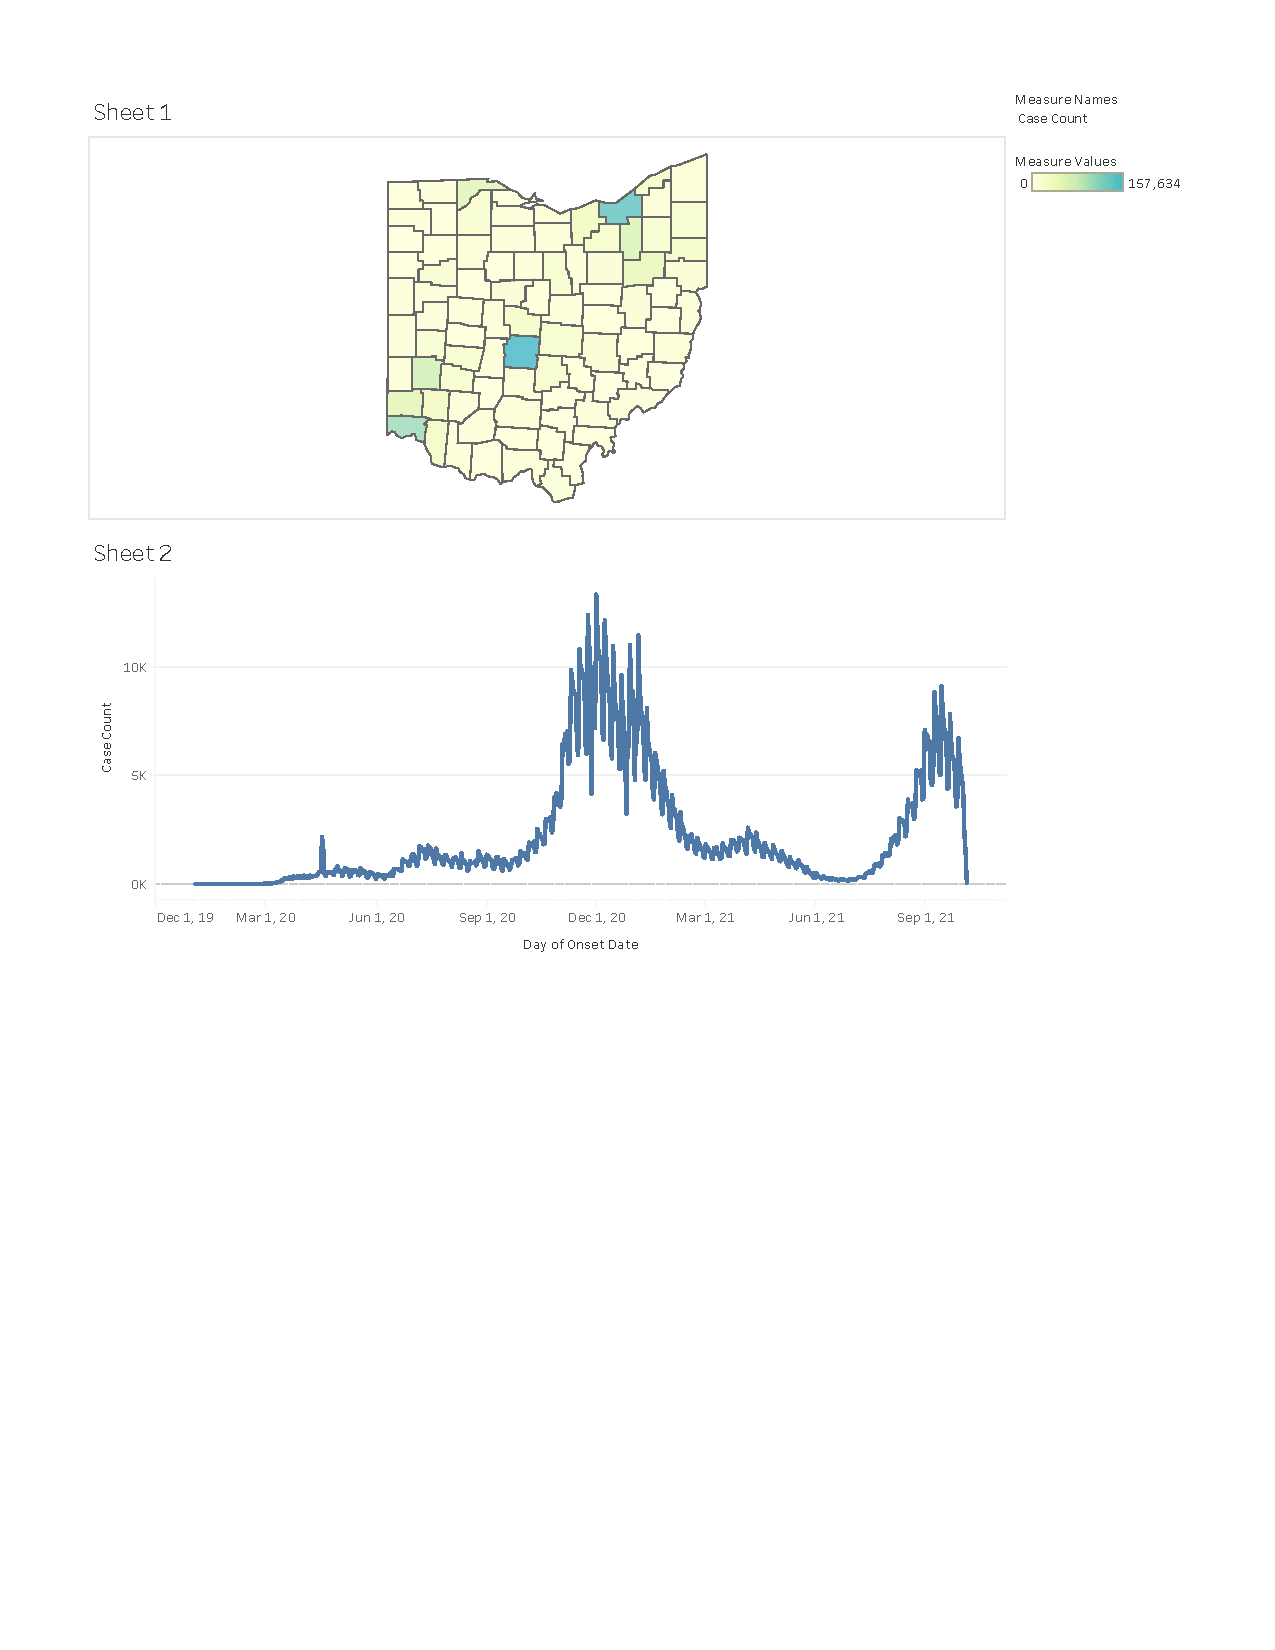
\includegraphics[width=0.8\textwidth,frame, clip, trim={0.5in 4.5in 0.5in 0.5in} ]{../../figures/tableau_example.pdf}
\end{center}


\question[0] Let us use both R and Python to quickly examine the \href{https://miamioh.instructure.com/courses/179812/files/25728247?module_item_id=4056689}{portmap\_sampled.csv}. The goal of using both R and Python is to expose you to libraries that allow for quick visualizations for the purpose of data exploration. \textbf{Recall that} visualizations should serve a specific purpose as highlighted in \href{https://fmegahed.github.io/isa401/fall2022/class13/13_fundamentals_data_viz.html?panelset4=activity5&panelset5=activity6&panelset6=activity7&panelset7=activity8#6}{Slide 6 of Class 13}.

\vspace{2in}

\question[0] If we were to discuss the grammar of graphics, the visualization below is helpful. The \href{https://englelab.gatech.edu/useRguide/introduction-to-ggplot2.html}{ENGE LAB: ggplot2} is an excellent introductory reference on the topic.

\begin{center}
	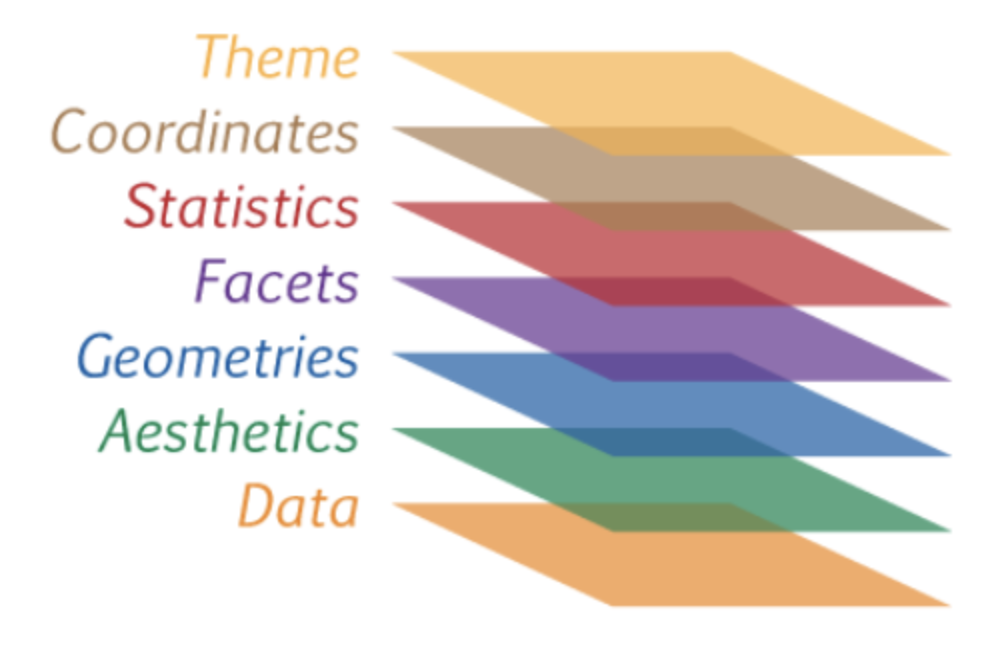
\includegraphics[width=0.8\textwidth,frame]{../../figures/gg_layers_from_gatech_englelab.png}
\end{center}

\end{questions}
\end{document}
